 In the previous chapter, we've seen that mining is based on SHA256 and we've analyzed the consequences if SHA256 is broken. In this chapter, we'll try to find some weaknesses in mining and use them to fool the process.

\section{Double-spending}

One of the very famous technic to trick a seller is called double-spending. As explained in \cite{double_spending_def}, a double-spending attack is used by a buyer to foul the seller, following the next steps :

\begin{enumerate}
  \item The buyer A broadcasts a transaction AB in the network where he pays seller B.
  \item The buyer A creates another block with a transaction $\overline{AB}$ which invalidates transaction AB.
  \item The buyer A secretly mines a branch on this new block.
  \item The buyer A waits that seller B sends his product.
  \item Once the buyer's branch is long enough, he broadcasts it which will deny transaction AB.
\end{enumerate}

With this method, the attacker uses his bitcoin twice, that's why it's called double-spending. \newline

\begin{figure}[h]
\centering
\captionsetup{justification=centering}
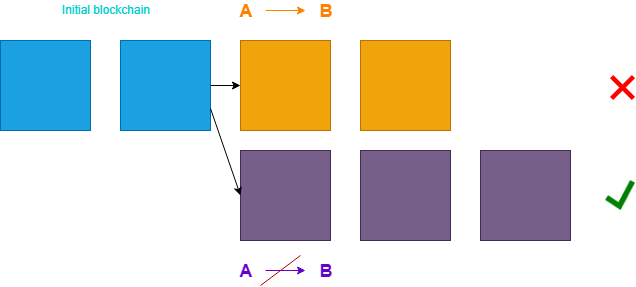
\includegraphics[width=8cm]{Figures/doubleSpending}
\caption{Double-spending - The longest chain will the purple one which invalidates the bitcoins sent to B while the seller has already sent his product}
\end{figure}
\medskip

\section{51\% attack}

  \subsection{What is it?}

The main difficulty to achieve this attack is to be able to build a longer chain to invalidate the transaction which gives bitcoins to the seller. One possible solution is the 51\% attack.

The 51\% attack has always been an important concern about blockchains' security. The main idea is that an attacker will control the majority of the computational power, i.e. at least 51\%.

\clearpage

\begin{pquotation}{Bitcoin glossary \cite{51Percent_definition}}
The ability of someone controlling a majority of the network hash rate to revise transaction history and prevent new transactions from confirming.
\end{pquotation}

In other words, an adversary with at least 51\% of the network will be able :

\begin{itemize}
  \item To prevent some users to do transactions, by systematically denying their transactions. Because the attacker controls the majority of the network, even if some nodes confirm the user's transaction, it will never be part of the longest chain.
  \item To reverse his transactions, this is double-spending.
\end{itemize}

  \subsection{Is it possible to implement it?}

    \paragraph{For Bitcoin}

To set a 51\% attack up, an attacker needs to gather enough mining computers to get more than 50\% of the computational power of the actual network.

Moreover, the attacker will have to supply enough electrical power to run those computers. \newline

Now, the real question is how much will it cost. We can try to estimate the cost for Bitcoin (see \cite{cost_bitcoin_51_attack}). \newline

First, buying specialized computers for mining will cost about \$2.4 million and \$250 million in infrastructure to install these computers and the equipment needed (like ventilation). \newline

Then, to power this structure, one will need around 30 Terawatts of electricity per year. For example, Morocco consumed 29 Terawatts in 2017 and Switzerland consumed 63 Terawatts the same year. All this electricity will cost around \$2 million by day. \newline

To sum up, a 51\% attack against Bitcoin will cost \$1.4 billion. This makes the attack almost impossible due to this huge cost, even for a government such as China (which is one of the biggest economies in the world), it will be very complicated to set up this attack.

    \paragraph{What about other blockchains?}


We've studied the feasibility of Bitcoin which is one of the most famous blockchains nowadays and its network is now very large. But one can wonder if the threat is more important with smaller blockchains. \newline

Indeed, the cost for a 51\% attack decreases for smaller coins. However, for every serious blockchain, there are still thousands or millions of nodes and anyways, it would more profitable to mine honestly and win coins through rewards.

On \href{https://www.crypto51.app/}{Crypto51}, we can observe the cost to make a 51\% attack on different cryptocurrencies. \newline

\begin{figure}[h]
\centering
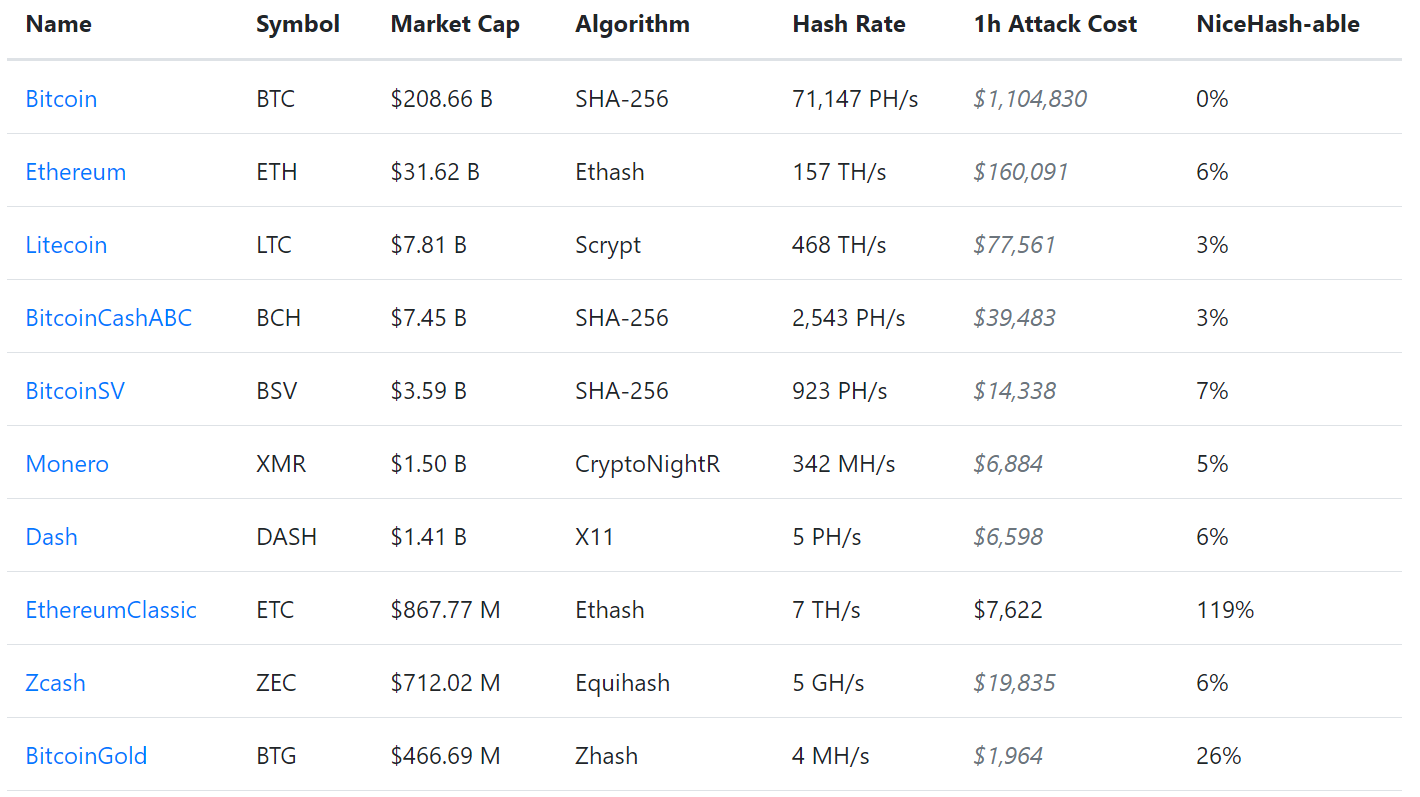
\includegraphics[width=8cm]{Figures/crypto51}
\caption{Crypto51}
\end{figure}
\medskip


Then, the probability remains low especially for the biggest blockchains. However, it can still happen (see \cite{blockchains_51_attack}). For example, EthereumClassic was attacked in January 2019 and it lost almost \$1.1 million in one day.

Preventing this attack can be very complicated but there are still some ideas :

\begin{itemize}
  \item Merging mining. Smaller cryptocurrencies can use mining power of larger ones so they become less vulnerable.
  \item Penalizing delayed blocks. The attacker mines blocks secretly and broadcasts them lately, a penalty will reduce the benefit of the attack.
  \item A detection algorithm for the 49\% left. Once the attack is detected, the 49\% left can try to acquire more power to stop the attack.
\end{itemize}
